\documentclass{beamer}
%% \documentclass[handout]{beamer}

\usetheme{default}

\usepackage[english]{babel}
\usepackage[latin1]{inputenc}

\usepackage{times}
\usepackage[T1]{fontenc}

%%
%%  some useful macro definitions & configuration settings
%%

\usepackage{latexsym}
\usepackage{graphicx}
\usepackage{url}
\usepackage{alltt}              % code examples with nicely formatted comments
\usepackage{xcolor}
\usepackage{pifont}
\usepackage{xspace}
\usepackage{array,booktabs}

\definecolor{quietred}{rgb}{.6,.2,.1}
\definecolor{quietblue}{rgb}{.1,.2,.7}
\definecolor{brightred}{rgb}{.9,0,.1}

%% > plot(x,y)      \REM{this produces a scatterplot}
\newcommand{\REM}[1]{\textsf{\small\color{quietred}\# #1}}

%% nice colour for R output: \begin{Rout} .. \end{Rout}
\newenvironment{Rout}{%
  \begin{footnotesize}\color{quietblue}\bfseries}{%
  \color{black}\mdseries\end{footnotesize}}

%% ... This is something \h{important}. ...
\newcommand<>{\h}[1]{\textbf#2{\color#2{quietred}#1}}
\newcommand<>{\hh}[1]{\textbf#2{\color#2{brightred}#1}}

%% cite \textcite{some text} in roman italic font
\newcommand{\textcite}[1]{\textrm{\textit{#1}}}

%% how can you live without the arrow (\so) and the hand (\hand) ?
\newcommand{\so}{\ding{234}\xspace}
\newcommand{\So}{\hh{\ding{229}}\xspace}
\newcommand{\hand}{\ding{43}\xspace}

%% \p{X=k};  \pC{X=k}{Y=l};  \bigp{X_i = k};   \pscale{\frac{Z}{S^2}};
%% probability P(X=k) and conditional probability P(X=k|Y=l), also with larger or scaled parentheses
%% \p[\theta]{X=k};  \pC[\text{interpolated}]{X=k}{Y=l};  ...
%% with optional subscripts (for model probability, null probability, etc.)
\newcommand{\p}[2][]{\mathop{\text{Pr}_{#1}}(#2)}
\newcommand{\pscale}[2][]{\mathop{\text{Pr}_{#1}}\!\left(#2\right)}
\newcommand{\bigp}[2][]{\mathop{\text{Pr}_{#1}}\bigl(#2\bigr)}
\newcommand{\pC}[3][]{\p[#1]{#2\,|\,#3}} 
\newcommand{\pCscale}[3][]{\pscale[#1]{#2\left|\,#3\right.\!}} 
\newcommand{\bigpC}[3][]{\bigp[#1]{#2\bigm|#3}} 

%% \Exp{X};  \Var{X};  \Exp[0]{X};  \Var[0]{X};  
%% \bigExp{X}; \bigVar{X}; \Expscale{X};  \Varscale{X};
%% expectation E[X] and variance V[X], expectation and variance under null hypothesis, 
%% and variants with largeer or scaled brackets
\newcommand{\Exp}[2][]{\text{E}_{#1}[#2]}
\newcommand{\Var}[2][]{\mathop{\text{Var}}_{#1}[#2]}
\newcommand{\bigExp}[2][]{\text{E}_{#1}\!\bigl[#2\bigr]}
\newcommand{\bigVar}[2][]{\mathop{\text{Var}}_{#1}\bigl[#2\bigr]}
\newcommand{\Expscale}[2][]{\text{E}_{#1}\left[#2\right]}
\newcommand{\Varscale}[2][]{\mathop{\text{Var}}_{#1}\left[#2\right]}


\title[SIGIL: Collocations 2]{Statistical Analysis of Corpus Data with R}
\subtitle{\emph{You shall know a word by the company it keeps!}\\
  Collocation extraction with statistical association measures\\
  --- Part 2 ---}

\author[Baroni \& Evert]{Designed by Marco Baroni\inst{1} and Stefan Evert\inst{2}}
\institute{
  \inst{1}Center for Mind/Brain Sciences (CIMeC)\\
  University of Trento
  \and
  \inst{2}Institute of Cognitive Science (IKW)\\
  University of Onsabr�ck
}
\date{}


\begin{document}

\frame{\titlepage}

 \begin{frame}
   \frametitle{Outline}
   \tableofcontents
 \end{frame}

%%%%%%%%%%%%%%%%%%%%%%%%%%%%%%%%%%%%%%%%%%%%%%%%%%%%%%%%%%%%%%%%%%%%%%%%

\section{Scaling up: working with large data sets}

\begin{frame}[fragile]
  \frametitle{Scaling up}

  \begin{itemize}
  \item We know how to compute association scores ($X^2$, Fisher, and $\log
    \theta$) for individual contingency tables now \ldots\pause
  \item[] \ldots\ but we want to do it automatically for 24,000 bigrams in the
    Brown data set, or an even larger number word pairs%
    \pause
  \item Of course, you can write a loop (if you know C/Java):
  \end{itemize}
  
\begin{verbatim}
> attach(Brown)
> result <- numeric(nrow(Brown))
> for (i in 1:nrow(Brown)) {
    if ((i %% 100) == 0) cat(i, " bigrams done\n")
    A <- rbind(c(O11[i],O12[i]), c(O21[i],O22[i]))
    result[i] <- chisq.test(A)$statistic
  }
\end{verbatim}

  \begin{itemize}
  \item[] \hand \verb|fisher.test()| is even slower \ldots
  \end{itemize}
\end{frame}

\begin{frame}
  \frametitle{Vectorising algorithms}

  \begin{itemize}
  \item Standard iterative algorithms (loops, function calls)\\
    are excruciatingly slow in R
    \begin{itemize}
    \item R is an interpreted language designed for interactive work and small
      scripts, not for implementing complex algorithms
    \end{itemize}
  \item Large amounts of data can be processed efficiently with \h{vector} and
    \h{matrix} operations \so vectorisation
    \begin{itemize}
    \item even computations involving millions of numbers are carried out
      instantaneously
    \end{itemize}
  \item How do you store a vector of contingency tables?
  \item[]\pause
  \item[\hand] as vectors $O_{11}$, $O_{12}$, $O_{21}$, $O_{22}$ in a data frame
  \end{itemize}
\end{frame}

\begin{frame}
  \frametitle{Vectorising algorithms}

  \begin{itemize}
  \item High-level functions like \texttt{chisq.test()} and
    \texttt{fisher.test()} cannot be applied to vectors
    \begin{itemize}
    \item only accept a single contingency table
    \item or vectors of cross-classifying factors from which a contingency
      table is built automatically
    \end{itemize}
  \item[]\pause
  \item Need to implement association measures ourselves
    \begin{itemize}
    \item i.e.\ calculate a test statistic or effect-size estimate\\
      to be used as an association score
    \end{itemize}
    \so have to take a closer look at the statistical theory 
  \end{itemize}
\end{frame}

\AtBeginSection[]{
  \begin{frame}<beamer:1| handout:0>
    \frametitle{Outline}
    \tableofcontents[current,currentsection]
  \end{frame}}

\AtBeginSubsection[]{
  \begin{frame}<beamer:1| handout:0>
    \frametitle{Outline}
    \tableofcontents[current,currentsubsection]
  \end{frame}}

%%%%%%%%%%%%%%%%%%%%%%%%%%%%%%%%%%%%%%%%%%%%%%%%%%%%%%%%%%%%%%%%%%%%%%%%

\subsection{Statistical association measures}

\begin{frame}
  \frametitle{Observed and expected frequencies}
  
  \begin{center}
    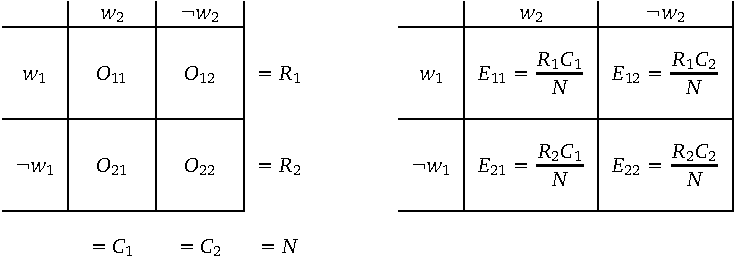
\includegraphics[width=\textwidth]{img/cont_table_observed_expected}
  \end{center}

  \begin{itemize}
  \item $R_1, R_2$ are the \h{row sums} ($R_1$ = marginal frequency $f_1$)
  \item $C_1, C_2$ are the \h{column sums} ($C_1$ = marginal frequency $f_2$)
  \item $N$ is the \h{sample size}
  \item $E_{ij}$ are the \h{expected frequencies} under independence $H_0$
  \end{itemize}
\end{frame}

\begin{frame}[fragile]
  \frametitle{Adding marginals and expected frequencies in R}

  \begin{alltt}
\REM{first, keep R from performing integer arithmetic}
> Brown <- transform(Brown,
  O11=as.numeric(O11), O12=as.numeric(O12),
  O21=as.numeric(O21), O22=as.numeric(O22))

> Brown <- transform(Brown,
  R1=O11+O12, R2=O21+O22,
  C1=O11+O21, C2=O12+O22,
  N=O11+O12+O21+O22)

\REM{we could also have calculated them laboriously one by one:}
Brown\$R1 <- Brown\$O11 + Brown\$O12 \REM{etc.}
\pause
> Brown <- transform(Brown,
  E11=(R1*C1)/N, E12=(R1*C2)/N,
  E21=(R2*C1)/N, E22=(R2*C2)/N)
\REM{now check that E11, \ldots, E22 always add up to N!}
  \end{alltt}
\end{frame}

\begin{frame}
  \frametitle{Statistical association measures}
  \framesubtitle{Measures of significance}

  \begin{itemize}
  \item Statistical association measures can be calculated from the observed,
    expected and marginal frequencies%
    \pause
  \item E.g.\ the chi-squared statistic $X^2$ is given by
    \[
    \text{\h{chi-squared}} =
    \sum_{ij} \frac{(O_{ij} - E_{ij})^2}{E_{ij}}
    \]
    (you can check this in any statistics textbook)%
    \pause
  \item The \texttt{chisq.test()} function uses a different version with
    Yates' continuity correction applied:
    \[
    \text{\h{chi-squared$_{\text{corr}}$}} =
    \frac{
      N \bigl( | O_{11}O_{22} - O_{12} O_{21} | - N/2 \bigr)^2
    }{
      R_1 R_2 C_1 C_2
    }
    \]
  \end{itemize}
\end{frame}

\begin{frame}
  \frametitle{Statistical association measures}
  \framesubtitle{Measures of significance}

  \begin{itemize}
  \item P-values for Fisher's exact test are rather tricky (and
    computationally expensive)
  \item Can use likelihood ratio test statistic $G^2$, which is less sensitive
    to small and skewed samples than $X^2$\\
    (Dunning 1993, 1998; Evert 2004)
    \begin{itemize}
    \item $G^2$ uses same scale (asymptotic $\chi^2_1$ distribution) as $X^2$,\\
      but you will notice that scores are entirely different
    \end{itemize}
  \end{itemize}
  \vspace{5mm}
  \[
  \text{\h{log-likelihood}} =
  2 \sum_{ij} O_{ij} \log {\frac {O_{ij}}{E_{ij}}}
  \]
\end{frame}

\begin{frame}[fragile]
  \frametitle{Significance measures in R}

  \begin{alltt}
\REM{chi-squared statistic with Yates' correction}
> Brown <- transform(Brown,
    chisq = N *
    (abs(O11*O22 - O12*O21) - N/2)^2 /
    (R1 * R2 * C1 * C2)
  )

\REM{Compare this to the output of \texttt{chisq.test()} for some bigrams.}
\REM{What happens if you do not apply Yates' correction?}
\pause
> Brown <- transform(Brown,
  logl = 2 * (
    O11*log(O11/E11) + O12*log(O12/E12) +
    O21*log(O21/E21) + O22*log(O22/E22)
  ))

> summary(Brown\$logl)  \REM{do you notice anything strange?}
  \end{alltt}
\end{frame}

\begin{frame}[fragile]
  \frametitle{Significance measures in R}
  \framesubtitle{Watch your numbers!}

  \begin{itemize}
  \item $\log 0$ is undefined, so $G^2$ cannot be calculated if any of the
    observed frequencies $O_{ij}$ are zero
    \begin{itemize}
    \item Why are the expected frequencies $E_{ij}$ unproblematic?
    \end{itemize}
    \pause
  \item For these terms, we can substitute $0 = 0\cdot \log 0$
  \end{itemize}

\begin{alltt}
> Brown <- transform(Brown,
  logl = 2 * (
    ifelse(O11>0, O11*log(O11/E11), 0) + 
    ifelse(O12>0, O12*log(O12/E12), 0) + 
    ifelse(O21>0, O21*log(O21/E21), 0) + 
    ifelse(O22>0, O22*log(O22/E22), 0)
  ))
\REM{\texttt{ifelse()} is a vectorised \texttt{if}-conditional}
\end{alltt}
\end{frame}


\begin{frame}
  \frametitle{Effect-size measures}

  \begin{itemize}
  \item Direct implementation allows a wide variety of effect size measures to
    be calculated
    \begin{itemize}
    \item but only direct maximum-likelihood estimates,\\
      confidence intervals are too complex (and expensive)
    \end{itemize}
  \item Mutual information and Dice coefficient give two different
    perspectives on collocativity:
    \[
    \text{\h{MI}} = \log_2 \frac{O_{11}}{E_{11}} \qquad
    \text{\h{Dice}} = \frac{2 O_{11}}{R_1 + C_1} 
    \]
  \item Modified log odds ratio is a reasonably good estimator:
    \[
    \text{\h{odds-ratio}} = 
    \log \frac{
      (O_{11} + \frac{1}{2}) (O_{22} + \frac{1}{2})
    }{
      (O_{12} + \frac{1}{2}) (O_{21} + \frac{1}{2})
    }
    \]
  \end{itemize}
\end{frame}

\begin{frame}
  \frametitle{Further reading}

  \begin{itemize}
  \item There are many other association measures
    \begin{itemize}
    \item Pecina (2005) lists 57 different measures
    \item[]
    \end{itemize}
  \item Evert, S.\ (2008, in press). Corpora and collocations.\\
    {\small\color{quietblue} In A.~L{\"u}deling and M.~Kyt{\"o} (eds.), {\em
        Corpus Linguistics.  An International Handbook}, article~57. Mouton de
      Gruyter, Berlin.}
    \begin{itemize}
    \item explains characteristic properties of the measures
    \item contingency tables for textual and surface cooccurrences
    \end{itemize}
  \item Evert, Stefan (2004). \emph{The Statistics of Word Cooccurrences: Word
      Pairs and Collocations}.\\
    {\small\color{quietblue} Dissertation, Institut f{\"u}r maschinelle
      Sprachverarbeitung, University of Stuttgart.  Published in 2005, URN
      urn:nbn:de:bsz:93-opus-23714.}
    \begin{itemize}
    \item full sampling models and detailed mathematical analysis
    \end{itemize}
  \item Online repository: \h{\url{www.collocations.de/AM}}
    \begin{itemize}
    \item with reference implementations in the UCS toolkit software
    \item[]
    \end{itemize}
  \item[\hand] all these sources use the notation introduced here
  \end{itemize}
\end{frame}

\begin{frame}[fragile]
  \frametitle{Implementiation of the effect-size measures}

  \begin{alltt}
\REM{Can you compute the association scores without peeking ahead?}
\pause
> Brown <- transform(Brown,
  MI = log2(O11/E11),
  Dice = 2 * O11 / (R1 + C1),
  log.odds = log(
    ((O11 + .5) * (O22 + .5)) /
    ((O12 + .5) * (O21 + .5))
  ))

\REM{check \texttt{summary(Brown)}: are there any more NA's?}
  \end{alltt}
\end{frame}

%%%%%%%%%%%%%%%%%%%%%%%%%%%%%%%%%%%%%%%%%%%%%%%%%%%%%%%%%%%%%%%%%%%%%%%%

\subsection{Sorting and ranking data frames}

\begin{frame}
  \frametitle{How to use association scores}

  \begin{itemize}
  \item Goal: use association scores to identify ``true'' collocations
  \item[]\pause
  \item \h{Strategy 1}: select word pairs with score above threshold
    \begin{itemize}
    \item no theoretically motivated thresholds for effect size
    \item significance thresholds not meaningful for collocations\\
      (How many bigrams are significant with $p < .001$?)
    \item alternative: take $n = 100, 500, 1000, \ldots$ highest-scoring word
      pairs \so \h{n-best list} (empirical threshold)
    \end{itemize}
  \item[]\pause
  \item \h{Strategy 2}: rank word pairs by association score
    \begin{itemize}
    \item reorder data frame by decreasing association scores
    \item word pairs at the top are ``more collocational''
    \item corresponds to n-best lists of arbitrary sizes
    \end{itemize}
  \end{itemize}
\end{frame}

\begin{frame}[fragile]
  \frametitle{Rankings in R}

  \begin{alltt}
> sum(Brown$chisq > qchisq(.999,df=1)) \REM{\(p < .001\)}
> sum(Brown$logl > qchisq(.999,df=1))

> Brown <- transform(Brown,
  r.logl = rank(-logl),  \REM{rank by \emph{decreasing} score}
  r.MI   = rank(-MI, ties="min"), \REM{see \texttt{?rank}}
  r.Dice = rank(-Dice, ties="min"))

> subset(Brown, r.logl <= 20, \REM{20-best list for log-likelihood}
  c(word1,word2,O11,logl,r.logl,r.MI,r.Dice))

\REM{Now do the same for MI and Dice.  What are your observations?}  

\REM{How many anti-collocations are there among the 100 most}
\REM{collocational bigrams according to log-likelihood?}
  \end{alltt}
\end{frame}

\begin{frame}[fragile]
  \frametitle{Sorting data frames in R}

  \begin{alltt}
> x <- 10 * sample(10) \REM{10, 20, \ldots, 100 in random order}

> sort(x)  \REM{sorting a vector is easy (default: ascending)}
> sort(x, decreasing=TRUE)

\REM{But for sorting a data frame, we need an index vector that tell us}
\REM{in what \emph{order} to rearrange the rows of the table.}

> sort.idx <- order(x)  \REM{also has \texttt{decreasing} option}
> sort.idx
> x[sort.idx]
  \end{alltt}
\end{frame}

\begin{frame}[fragile]
  \frametitle{Sorting data frames in R: practice time}

  \begin{alltt}
\REM{try to sort bigram data set by log-likelihood measure}
\pause
> sort.idx <- order(Brown\$logl, decreasing=TRUE)
> Brown.logl <- Brown[sort.idx, ]

> Brown.logl[1:20, 1:6]

\REM{Now construct a simple character vector with the first 100 bigrams,}
\REM{or show only relevant columns of the data frame for the first 100 rows.}

\REM{Show the first 100 noun-noun bigrams (\texttt{pos} code \texttt{N}) and}
\REM{the first 100 adjective-noun bigrams (codes \texttt{J} and \texttt{N}).}

\REM{If you know some programming, can you write a function that}
\REM{displays the first \(n\) bigrams for a selected association measure?}
  \end{alltt}
\end{frame}

\begin{frame}[fragile]
  \frametitle{Sorting data frames in R: practice time}
  \framesubtitle{Example solutions for practice questions}

  \begin{alltt}
> paste(Brown.logl\$word1, Brown.logl\$word2)[1:100]
> paste(Brown\$word1, Brown\$word2)[sort.idx[1:100]]

\REM{advanced code ahead: make your life easy with some R knowledge}
> show.nbest <- function(myData, 
  AM=c("chisq","logl","MI","Dice","O11"), n=20) \{
    AM <- match.arg(AM) \REM{allows unique abbreviations}
    idx <- order(myData[[AM]], decreasing=TRUE)
    myData[idx[1:n], c("word1","word2","O11",AM)]
  \}

> show.nbest(Brown, "chi")

\REM{Can you construct a table that compares the measures side-by-side?}
  \end{alltt}
\end{frame}

%%%%%%%%%%%%%%%%%%%%%%%%%%%%%%%%%%%%%%%%%%%%%%%%%%%%%%%%%%%%%%%%%%%%%%%%

\section{The evaluation of association measures}

\begin{frame}
  \frametitle{Evaluation of association measures}

  \begin{itemize}
  \item One way to achieve a better understanding of different association
    measures is to evaluate and compare their performance in \h{multiword
      extraction} tasks
    \begin{itemize}
    \item published studies include Daille (1994), Krenn (2000), Evert \&
      Krenn (2001, 2005), Pearce (2002) and Pecina (2005)
    \end{itemize}
    \pause
  \item ``Standard'' multiword extraction approach
    \begin{itemize}
    \item extract (syntactic) collocations from suitable text corpus
    \item rank according to score of selected association measure
    \item take $n$-best list as \h{multiword candidates}
    \item additional filtering, e.g.\ by frequency threshold
    \item candidates have to be validated manually by expert
    \end{itemize}
    \pause
  \item Evaluation based on manual validation
    \begin{itemize}
    \item expert marks candidates as true (TP) or false (FP) positive
    \item calculate \h{precision} of n-best list $= \#TP / n$
    \item if all word pairs are annotated, also calculate \h{recall}
    \end{itemize}
  \end{itemize}
\end{frame}

\begin{frame}
  \frametitle{The PP-verb data set of Krenn (2000)}

  \begin{itemize}
  \item Krenn (2000) used a data set of German PP-verb pairs to evaluate
    the performance of association measures
    \begin{itemize}
    \item goal: identification of lexicalised German PP-verb combinations such
      as \emph{zum Opfer fallen} (fall victim to),\\ \emph{ums Leben kommen}
      (lose one's life), \emph{im Mittelpunkt stehen} (be the centre of
      attention), etc.
    \item manual annotation distinguishes between support-verb constructions
      and figurative expressions (both are MWE)
    \item candidate data for original study extracted from 8 million word
      fragment of German \emph{Frankfurter Rundschau} corpus
    \end{itemize}
  \item PP-verb data set used in this session
    \begin{itemize}
    \item candidates extracted from full \emph{Frankfurter Rundschau} corpus
      (40 million words, July 1992 -- March 1993)
    \item more sophisticated syntactic analysis used
    \item frequency threshold $f\geq 30$ leaves 5102 candidates
    \end{itemize}
  \end{itemize}
\end{frame}

%%%%%%%%%%%%%%%%%%%%%%%%%%%%%%%%%%%%%%%%%%%%%%%%%%%%%%%%%%%%%%%%%%%%%%%%

\subsection{Precision/recall tables and graphs}

\begin{frame}
  \frametitle{Table of n-best precision values}

  \begin{itemize}
  \item Evaluation computes precision (and optionally) recall for various
    association measures and n-best lists
  \item[]
  \item[]
    \begin{center}\small
      \begin{tabular}{r || r | r | r | r | r | r | r}
        n-best & logl & chisq & t-score & MI  & Dice & odds & freq \\
        \hline
         100   & 42.0 & 24.0 &   38.0  & 19.0 & 21.0 & 17.0 & 27.0 \\
         200   & 37.5 & 23.5 &   35.0  & 16.5 & 19.5 & 14.0 & 26.5 \\
         500   & 30.4 & 24.6 &   30.2  & 18.0 & 16.4 & 19.6 & 23.0 \\
       1,000   & 27.1 & 23.9 &   28.1  & 21.6 & 14.9 & 24.4 & 19.2 \\
       1,500   & 25.3 & 25.0 &   24.8  & 24.3 & 13.2 & 25.3 & 18.0 \\
       2,000   & 23.4 & 23.4 &   21.9  & 23.1 & 12.6 & 23.3 & 16.3
      \end{tabular}
    \end{center}
  \item[]
  \item[]
  \item More intuitive presentation for arbitrary n-best lists in the form of
    \h{precision graphs} (or precision-recall graphs)
  \end{itemize}
\end{frame}

\begin{frame}
  \frametitle{Precision graphs}

  \begin{center}
    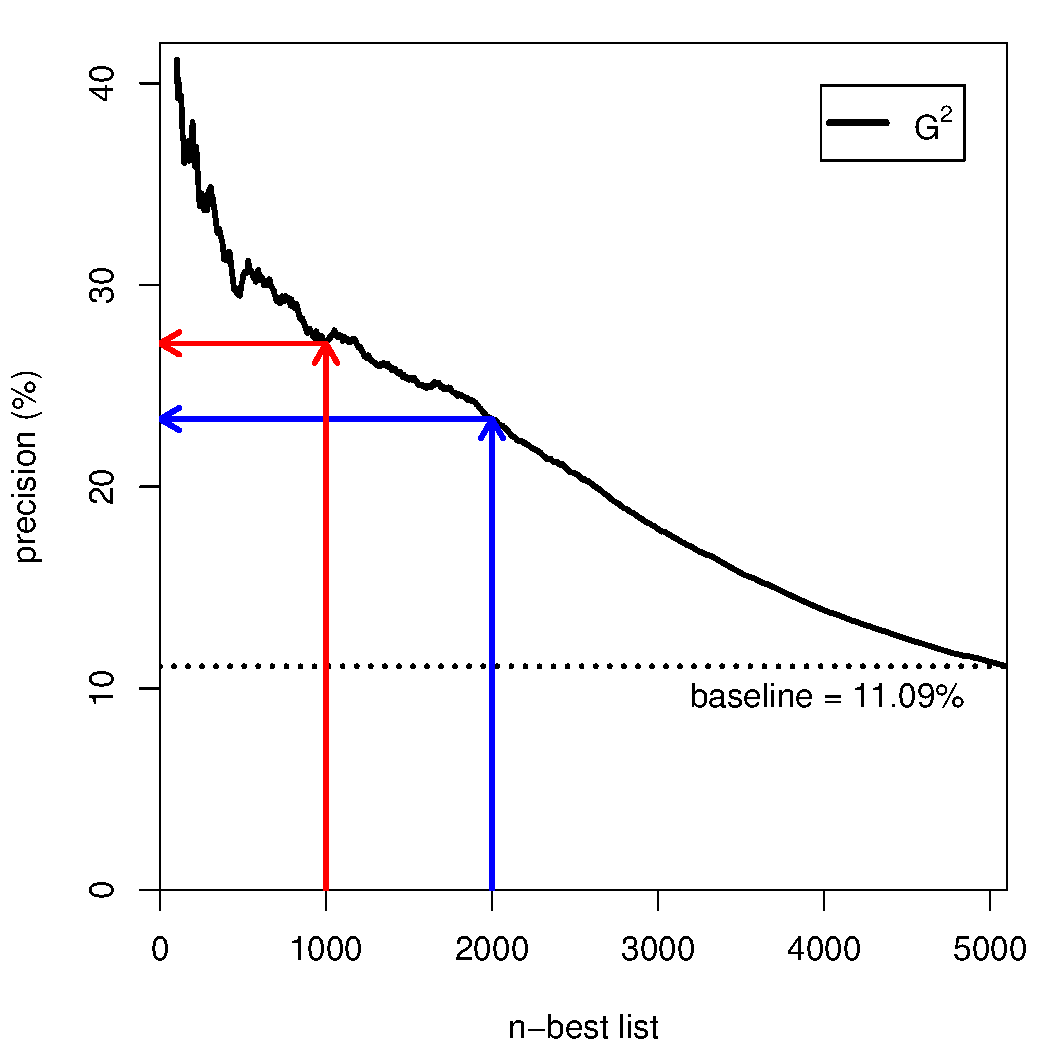
\includegraphics[width=8cm]{img/mwe_eval_illustration}
  \end{center}
\end{frame}

\begin{frame}
  \frametitle{Precision graphs}

  \begin{center}
    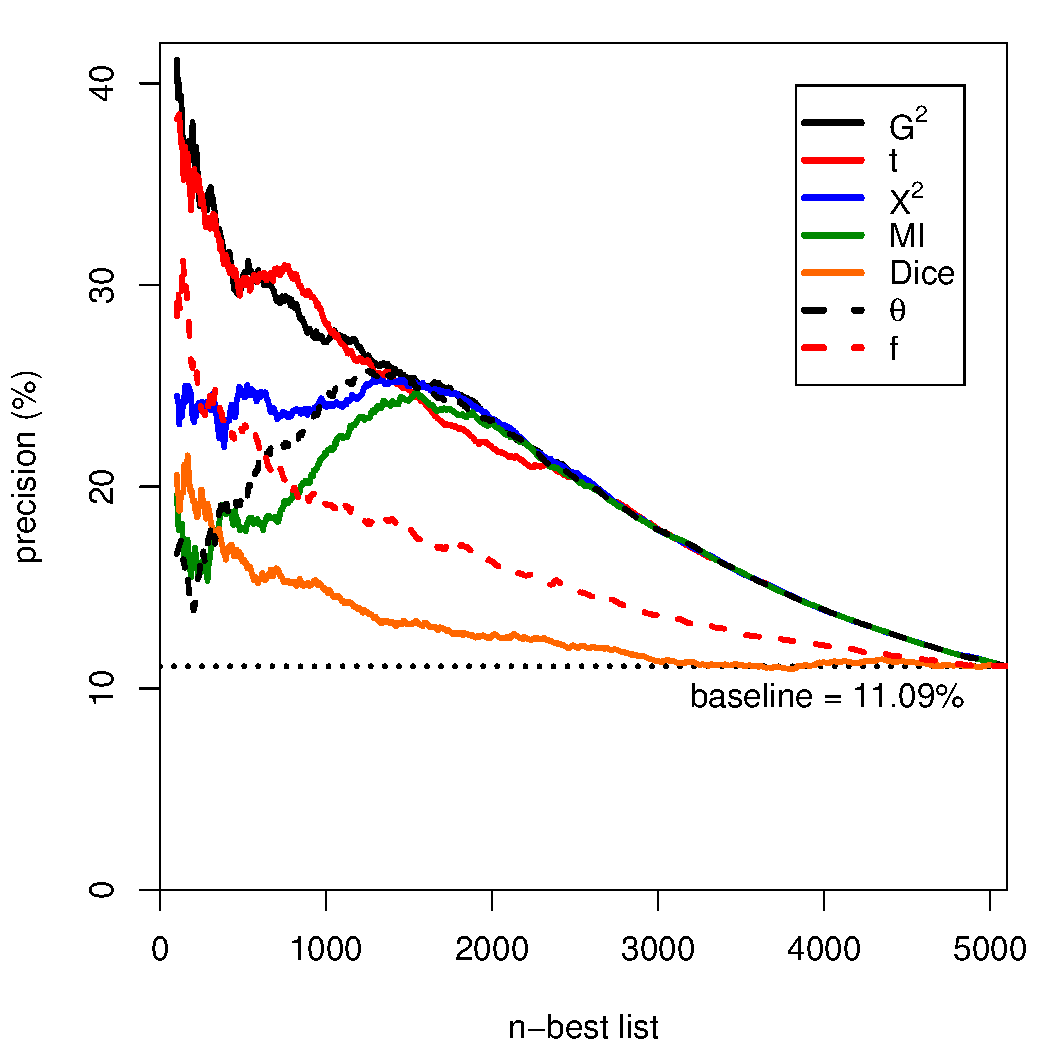
\includegraphics[width=8cm]{img/mwe_eval_1}
  \end{center}
\end{frame}

\begin{frame}
  \frametitle{Precision graphs: zooming in}

  \begin{center}
    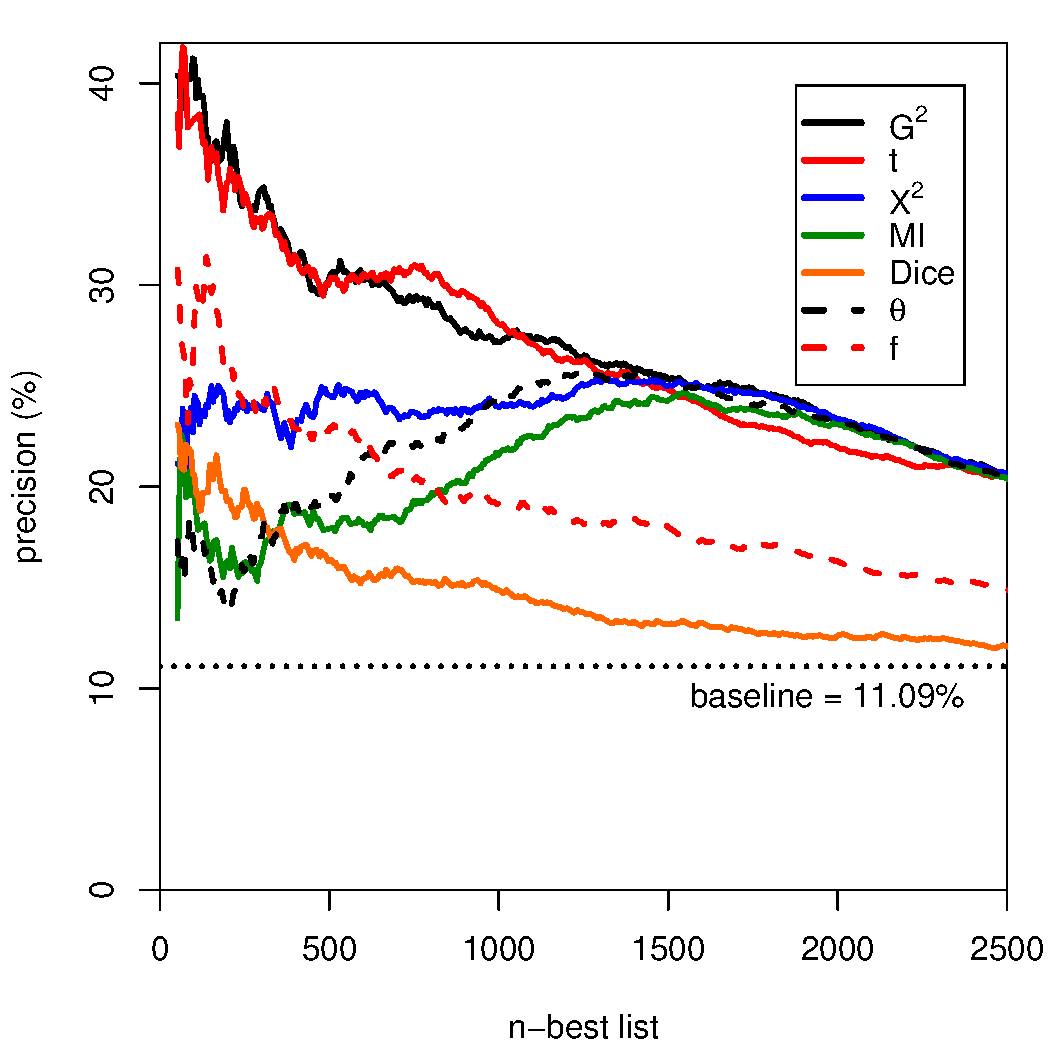
\includegraphics[width=8cm]{img/mwe_eval_2}
  \end{center}
\end{frame}

\begin{frame}
  \frametitle{Precision-by-recall graphs}

  \begin{center}
    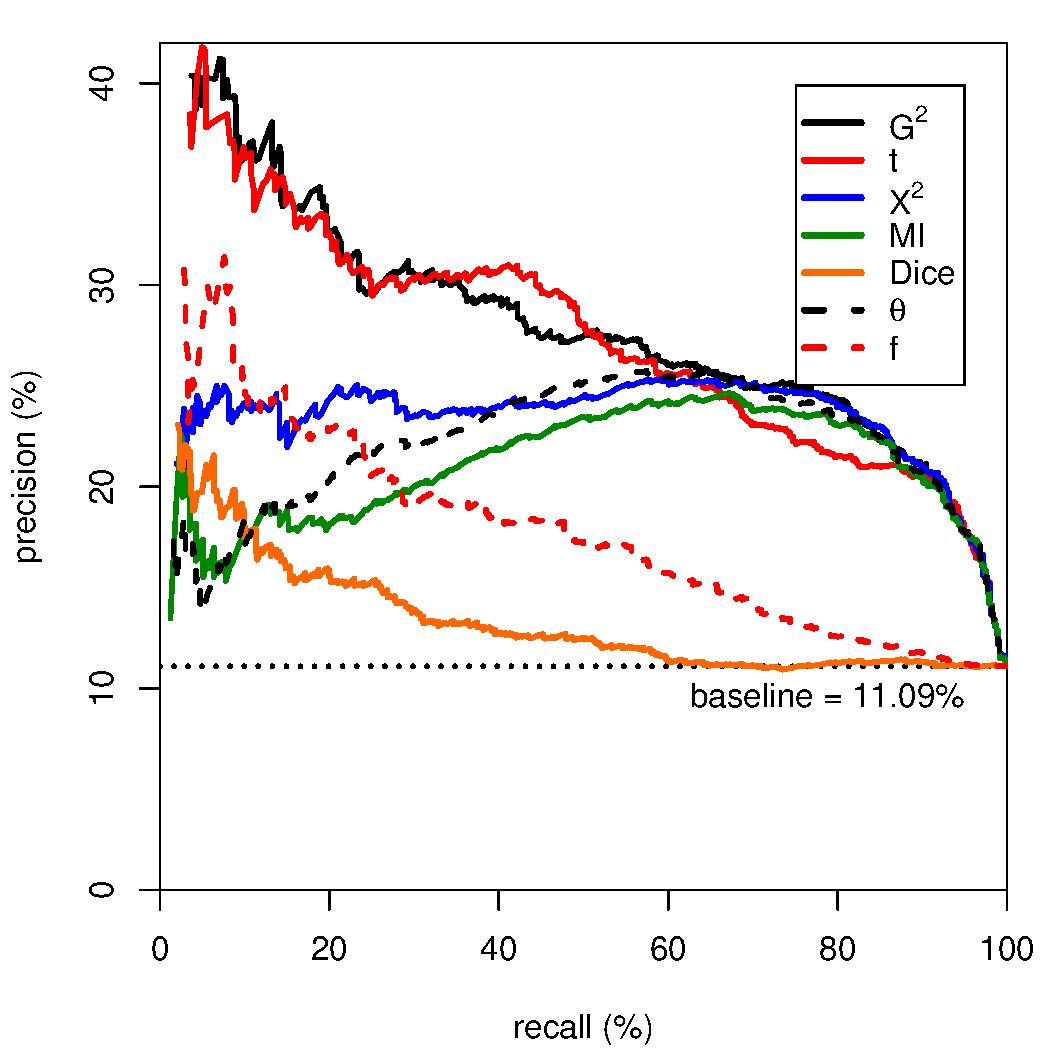
\includegraphics[width=8cm]{img/mwe_eval_3}
  \end{center}
\end{frame}

%%%%%%%%%%%%%%%%%%%%%%%%%%%%%%%%%%%%%%%%%%%%%%%%%%%%%%%%%%%%%%%%%%%%%%%%

\subsection{MWE evaluation in R}

\begin{frame}[fragile]
  \frametitle{The PP-verb data set}

  \begin{itemize}
  \item \verb|krenn_pp_verb.tbl| available from course homepage
  \item Data frame with 5102 rows and 14 columns:
    \begin{itemize}
    \item \h{PP} = prepositional phrase (lemmatised)
    \item \h{verb} = lexical verb (lemmatised)
    \item \h{is.colloc} = Boolean variable indicating TPs (= MWE)
    \item \h{is.SVC}, \h{is.figur} distinguish subtypes of MWE
    \item \h{freq}, \h{MI}, \h{Dice}, \h{z.score}, \h{t.score}, \h{chisq},
      \h{chisq.corr}, \h{log.like}, \h{Fisher} = precomputed association
      scores\\ (Do you recognise all association measures?)
    \end{itemize}
  \item[]
  \item Our goal is to reproduce the table and plots shown on the previous
    slides (perhaps not all the bells and whistles)
  \end{itemize}
\end{frame}

\begin{frame}[fragile]
  \frametitle{Precision tables: your turn!}

  \begin{alltt}
> PPV <- read.delim("krenn_pp_verb.tbl")
> colnames(PPV)

> attach(PPV)

\REM{You should now be able to sort the data set and calculate}
\REM{precision for some association measures and n-best lists.}
\REM{(hint: \texttt{sum()} counts TRUE entries in Boolean vector)}
  \end{alltt}
\end{frame}

\begin{frame}[fragile]
  \frametitle{Precision tables}

  \begin{alltt}
> idx.logl <- order(log.like, decreasing=TRUE)
> sum(is.colloc[idx.logl[1:500]]) / 500   \REM{\(n = 500\)}
> sum(is.colloc[idx.logl[1:1000]]) / 1000 \REM{\(n = 1000\)}

\REM{use \texttt{cumsum()} to calculate precision for all n-best lists}
> prec <- cumsum(is.colloc[idx.logl]) / 
  (1:nrow(PPV))
> prec[c(100,200,500,1000,1500,2000)]    
  \end{alltt}
\end{frame}

\begin{frame}[fragile]
  \frametitle{Precision tables: an elegant solution}

  \begin{alltt}
> show.prec <- function(myData, AM, n) \{
  stopifnot(AM \%in\% colnames(myData)) \REM{safety first!}
  sort.idx <- order(myData[[AM]], decreasing=TRUE)
  prec <- cumsum(myData\$is.colloc[sort.idx]) / 
          (1:nrow(myData))
  result <- data.frame(100 * prec[n]) \REM{percentages}
  rownames(result) <- n  \REM{add nice row/column labels}
  colnames(result) <- AM
  result  \REM{return single-column data frame with precision values}
  \}

> show.prec(PPV, "chisq", c(100,200,500,1000))

  \end{alltt}
\end{frame}

\begin{frame}[fragile]
  \frametitle{Precision tables: an elegant solution}

  \begin{alltt}
> n.list <- c(100,200,500,1000,1500,2000)

\REM{data frames of same height can be combined in this way}
> prec.table <- cbind(
    show.prec(PPV, "log.like", n.list),
    show.prec(PPV, "Fisher", n.list),
    show.prec(PPV, "chisq", n.list),
    show.prec(PPV, "chisq.corr", n.list),
    show.prec(PPV, "z.score", n.list),
    show.prec(PPV, "t.score", n.list),
    show.prec(PPV, "MI", n.list),
    show.prec(PPV, "Dice", n.list),
    show.prec(PPV, "freq", n.list)
  )

> round(prec.table, 1) \REM{rounded values are more readable}
  \end{alltt}
\end{frame}

\begin{frame}[fragile]
  \frametitle{Precision graphs}

  \begin{alltt}
\REM{first, generate sort index for each association measure}
> idx.ll <- order(log.like, decreasing=TRUE)
> idx.chisq <- order(chisq, decreasing=TRUE)
> idx.t <- order(t.score, decreasing=TRUE)
> idx.MI <- order(MI, decreasing=TRUE)
> idx.Dice <- order(Dice, decreasing=TRUE)
> idx.f <- order(freq, decreasing=TRUE)
 \end{alltt}
\end{frame}

\begin{frame}[fragile]
  \frametitle{Precision graphs}

  \begin{alltt}
\REM{second, calculate precision for all n-best lists}
> n.vals <- 1:nrow(PPV)

> prec.ll <- cumsum(is.colloc[idx.ll]) *
  100 /  n.vals
> prec.chisq <- cumsum(is.colloc[idx.chisq]) *
  100 / n.vals
> prec.t <- cumsum(is.colloc[idx.t]) *
  100 / n.vals
> prec.MI <- cumsum(is.colloc[idx.MI]) *
  100 / n.vals
> prec.Dice <- cumsum(is.colloc[idx.Dice]) *
  100 / n.vals
> prec.f <- cumsum(is.colloc[idx.f]) *
  100 / n.vals
  \end{alltt}
\end{frame}

\begin{frame}[fragile]
  \frametitle{Precision graphs}

  \begin{alltt}
\REM{increase font size, set plot margins (measured in lines of text)}
> par(cex=1.2, mar=c(4,4,1,1)+.1)

\REM{third: plot as line, then add lines for further measures}
> plot(n.vals, prec.ll, type="l", 
  ylim=c(0,42), xaxs="i", \REM{fit x-axis range tightly}
  lwd=2, col="black",     \REM{line width and colour}
  xlab="n-best list", ylab="precision (\%)")
> lines(n.vals, prec.chisq, lwd=2, col="blue")
> lines(n.vals, prec.t, lwd=2, col="red")
> lines(n.vals, prec.MI, lwd=2, col="black",
  lty="dashed") \REM{line type: solid, dashed, dotted, \ldots}
> lines(n.vals, prec.Dice, lwd=2, 
  col="blue", lty="dashed")
> lines(n.vals, prec.f, lwd=2, 
  col="red", lty="dashed")
  \end{alltt}
\end{frame}

\begin{frame}[fragile]
  \frametitle{Precision graphs}

  \begin{alltt}
\REM{add horizontal line for baseline precision}
> abline(h = 100 * sum(is.colloc) / nrow(PPV))

\REM{and legend with labels for the precision lines}
> legend("topright", inset=.05, \REM{easy positioning of box}
  bg="white", \REM{fill legend box so it may cover other graphics}
  lwd=2,      \REM{short vectors are recycled as necessary}
  col=c("black", "blue", "red"), 
  lty=c("solid","solid","solid", \REM{no default values here!}
        "dashed","dashed","dashed"),
  \REM{either string vector, or ``expression'' for mathematical typesetting}
  legend=expression(G^2, X^2, t, "MI", "Dice", f))
  \end{alltt}
\end{frame}

\begin{frame}
  \frametitle{Precision graphs: playtime}

  \begin{itemize}
  \item Add further decorations to plot (baseline text, arrows, \ldots)
  \item Write functions to simplify plot procedure
    \begin{itemize}
    \item you may want to explore \texttt{type="n"} plots
    \end{itemize}
  \item Precision values highly erratic for $n < 50$ \so don't show
  \item Graphs look smoother with thinning
    \begin{itemize}
    \item increment $n$ in steps of 5 or 10 (rather than 1)
    \end{itemize}
  \item Calculate recall and create precision-by-recall graphs
  \item[]
  \item[\hand] all those bells, whistles and frills are implemented in the UCS
    toolkit (\url{www.collocations.de/software.html})
  \end{itemize}
\end{frame}

\end{document}
